\documentclass{article}
\usepackage[utf8]{luainputenc}
\usepackage[T1]{fontenc}
\usepackage[a4paper,margin=0.75in, bottom=1in]{geometry}
\usepackage{listings}
\usepackage{minted}
\usepackage{courier}
\usepackage{amsmath}
\usepackage{enumerate}
\usepackage{graphicx}
\usepackage{hyperref}

\begin{document}
	
	\hrulefill
	\begin{center}
		\bfseries % Fettdruck einschalten
		\sffamily % Serifenlose Schrift
		\begin{huge}
			GTI: Grundlagen der Theoretischen Informatik
		\end{huge}\\
		\begin{Large}
			Sommersemester 2017, 1. Übungsblatt
		\end{Large}\\
		\begin{small}
			Christopher Husemann, Luis Herrmann; Tutor: Kristin Knorr; Mo 12:00-14:00
		\end{small}
		
		\vspace{-10pt}
	\end{center}
	\hrulefill
	
	\section*{Aufgabe 2 - \textit{Zustandsdiagramme}}
	\begin{enumerate}[a)]
		\item Gesucht ist eine Idee über alle Wörter, für die jeder dritte Buchstabe eine 0 ist. Trivialerweise sind auch jene Wörter enthalten, die weniger als 3 Buchstaben haben. Damit ist klar, dass der Initialzustand $S_\epsilon$ akzeptierend sein muss, ebenso die Zustände $S_{*1}$ und $S_{*2}$, welche für das Lesen eines bzw. zweier beliebiger weiterer Zeichen erreicht werden. Nehmen wir nun, es wird als nächstes eine 0 gelesen. Dann haben wir ein Wort der Länge 3, welches in der 3 endet, und der Automat landen im akzeptierenden Zustand $S_0$. Wird dagegen eine 1 gelesen, so kann das Wort nicht mehr in der Sprache liegen, egal welche Zeichen noch gelesen werden, und der Automat landet in einem "toten" nicht-akzeptierenden Zustand $S_3$, der für beliebige weitere Zeichen zu sich selbst überführt wird.
		
		Nehmen wir an, wir haben 3 Zeichen gelesen und das dritte war eine 0. Dann sind die nächsten zwei Zeichen unwichtig und der Automat wird unabhängig von dem gelesenen Zeichen zu den zählenden Zuständen $S_1$ und $S_2$ überführt, erst danach präsentiert sich wieder das vorherige Szenario und die Überführungsfunktion bildet entsprechend auf den akzeptierenden Zustand $S_0$ oder auf den toten Zustand $S_3$ ab.
		
		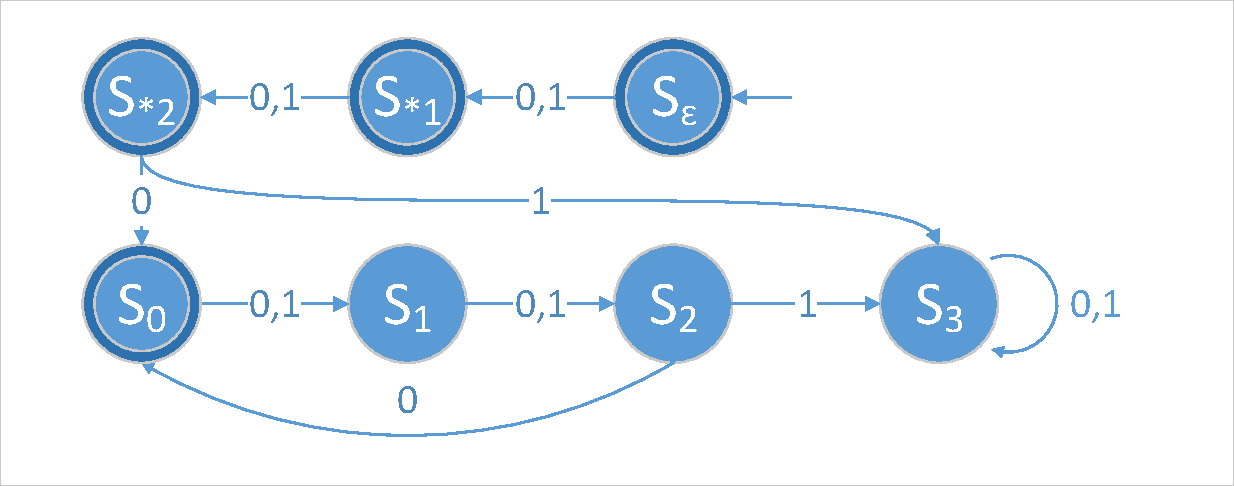
\includegraphics[width=\textwidth]{dfa1.pdf}
		\item Die nachfolgende dfa akzeptiert alle Bitwörter, die Länge mindestens drei haben und deren drittletzter Buchstabe eine 0 ist. Wir beginnen im ZUstand $S_1$. Nehmen wir an, wir lesen als erstes das Zeichen 1. Dann können wir im nicht-akzeptierenden Zustand $S_0$ verbleiben. Erst, sobald die erste 0 gelesen wird, ist zu prüfen, ob der String nach zwei weiteren eingegebenen Zeichen terminiert, denn dann haben wir gerade ein Wort aus der gegebenen Sprache gefunden. Dazu verzweigt sich die dfa zunächst in Zustände $S_{01}$ und $S_{00}$ und schließlich weiter in die akzeptierenden Zustände $F = S_{011}, S_{010}, S_{001}, S_{000}$, wobei durch diese Zutände alle möglichen 2-Bitfolgen nach der ersten 0 berücksichtigt werden.
		
		Nehmen wir nun an, dass nach der ersten 0 und den den darauffolgenden zwei Bits noch weitere Bits gelesen werden. Dann können wir abhängig von den zwei letzten gelesenen Zeichen zu dem entsprechenden Zustand des Automaten springen, der dem Suffix ab der nächsten 0 plus gelesenem Zeichen entspricht.
		
		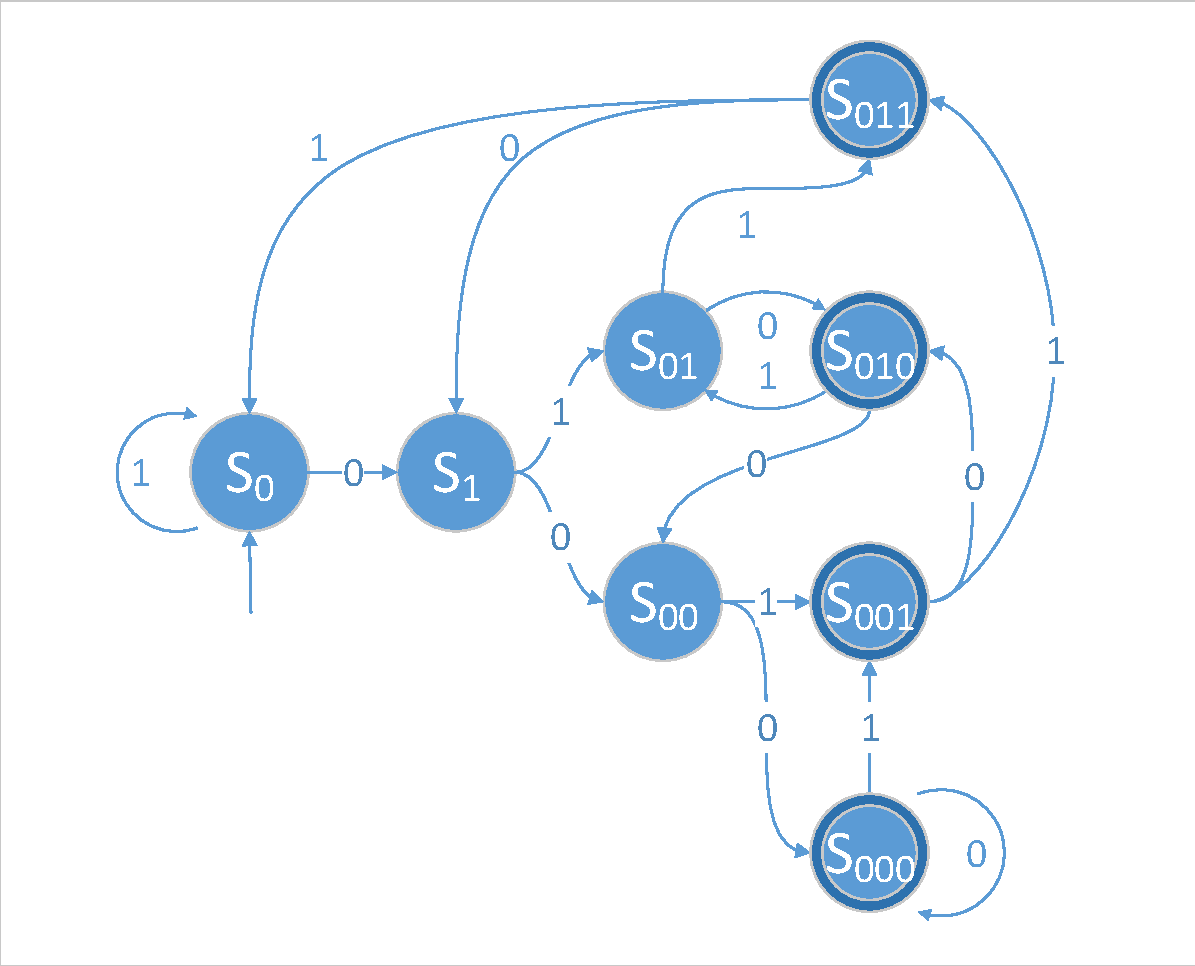
\includegraphics[width=\textwidth]{dfa2.pdf}
		
		\item Die nachfolgende dfa akzeptiert alle Bitwörter, in denen gleichviele Teilsequenzen 01 und 10 vorhanden sind. Die Idee ist folgende: Angenommen, das erste gelesene Zeichen ist eine 0. Solange keine 1 gelesen wird, gibt es 0 Teilsequenzen 01 und 0 Teilsequenzen 10, sodass das Wort trivialerweise in der Sprache leigt. daher sind bereits der Eingangszustand $S_i$ und der Eingangszustand $S_0$ akzeptierende Zustände. Nehmen wir nun an, wir lesen zum ersten Mal eine 1. Dann haben wir zum ersten Mal eine Teilsequenz 01 gelesen und müssen den akzeptierenden Zustand verlassen. Nun müssen wir so lange in dem nicht-akzeptierenden Zustand $S_{10}$ verbleiben, bis wir die nächste 0 lesen, denn dann haben wir gerade eine Sequenz 10 gefunden und die Anzahl der Teilsequenzen 10 und 01 ist somit ausgeglichen; wir können somit in den akzeptierenden Zustand $S_0$ zurückkehren und von neuem beginnen.
		
		Für den Fall, dass das erste gelesene Zeichen eine 1 ist, gelten symmetrische genau die gleichen Überlegungen.
		
		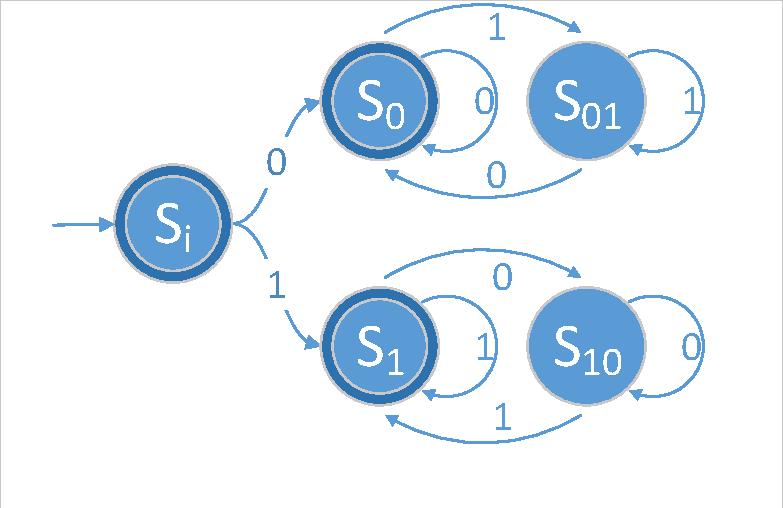
\includegraphics[width=0.6\textwidth]{dfa3.pdf}
		
		\item Die nächste dfa akzeptiert alle Bitwörter mit führender 1, die eine durch 5 teilbare natürlich Zahl binär kodieren. Wir wollen naheliegenderweise Zustände $S_0, S_1, S_2, S_3, S_4$ benutzen, sodass sich unsere Maschine nach Bearbeiten eines Bitwortes immer im Zustand der zugehörigen Äquivalenzklasse bezüglich der Operation $\textrm{mod} 5$ befindet. Die Konstruktion überlegt man sich am Besten induktiv. Angenommen, wir haben einen Automaten $A$ für besagte Sprache und nach Lesen eines Wortes der Länge $n$ befindet sich der Automat im Zustand $S_m$ mit $m:= \textrm{dec}(w)\; \textrm{mod} \; 5$. Dann gilt für das Wort $\tilde{w} := wx_{n+1}$, dass $x_{n+1} \in \{0,1\}$ und dementsprechend gilt für die kodierte Dezimalzahl, dass:
		\begin{equation}
		\textrm{dec}(\tilde{w}) = 2\textrm{dec}(w) + \textrm{dec}(x_{n+1})
		\end{equation}
		Somit sind 10 Fälle zu berücksichtigen:
		\begin{align}
		&(2\textrm{dec}(w)) \textrm{mod} 5 = \begin{cases}
		0,&m = 0\\ 2,&m = 1\\4,&m=2\\1,&m=3\\3,&m=4
		\end{cases}
		&& (2\textrm{dec}(w)+1)\textrm{mod} 5 = \begin{cases}
		1,&m=0\\3,&m=1\\0,&m=2\\2,&m=3\\4,&m=4
		\end{cases}
		\end{align}
		
		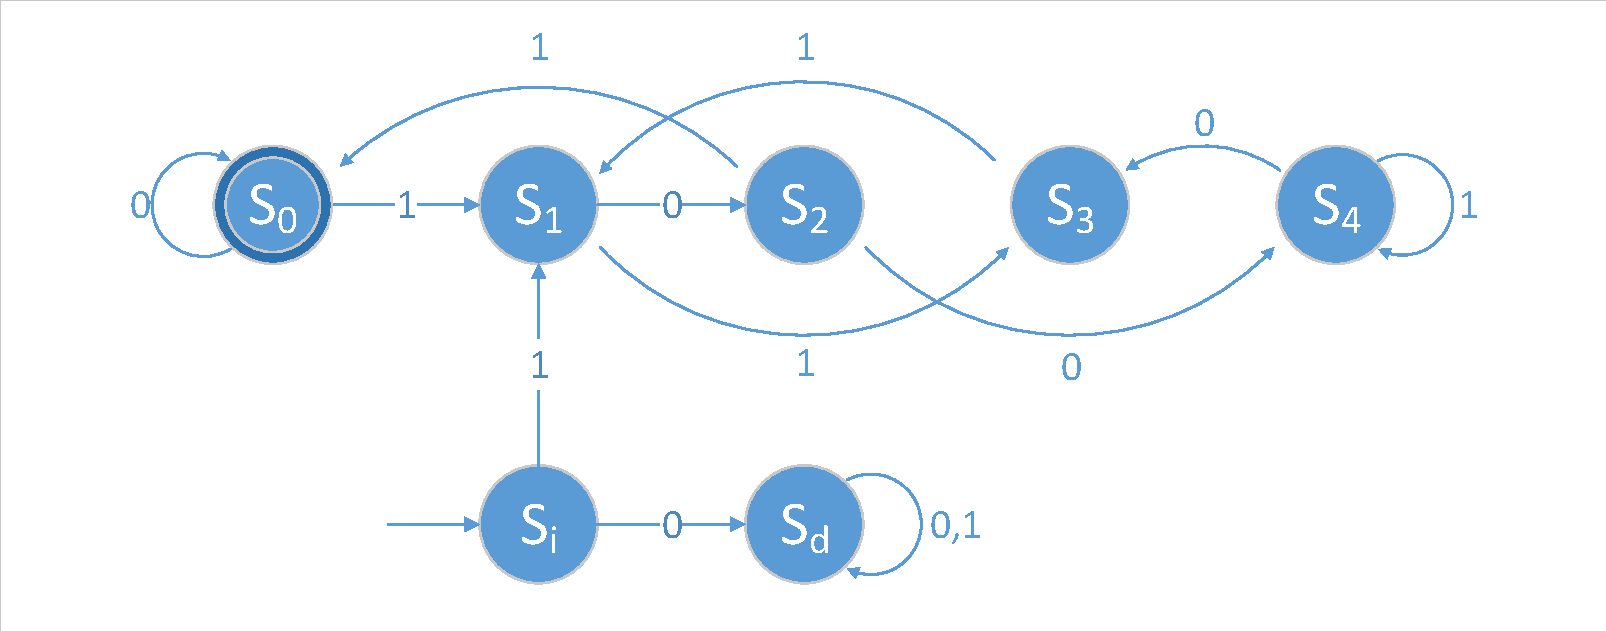
\includegraphics[width=\textwidth]{dfa4.pdf}
		
	\end{enumerate}
	
	
	\section*{Aufgabe 3 - \textit{Reguläre Ausdrücke I}}
	\begin{enumerate}
		\item Wir charakterisieren die Menge aller Wörter, für die jeder 3. Buchstabe eine 0 ist. Die zugehörige Sprache ist $L(\alpha)$, wobei $\alpha$ der reguläre Ausdruck ist:
		\begin{equation}
		\alpha = ((0 \cup 1)^20)^* (\epsilon \cup (0 \cup 1) \cup (0 \cup 1 )^2)
		\end{equation}
		Da der reguläre Ausdruck $((0 \cup 1)^20)^*$ insbesondere das leere Wort enthält, sind mit $(\epsilon \cup (0 \cup 1) \cup (0 \cup 1 )^2)$ auch jene Wörter der Länge $<3$ berücksichtigt, die trivialerweise in der Sprache enthalten sind.
		
		\item Die Menge aller Wörter, die min. Länge 3 haben und deren drittletzter Buchstabe eine 0 ist lässt sich als Sprache $L(\alpha)$ charakterisieren, wobei $\alpha$ der reguläre Ausdruck ist:
		\begin{equation}
		\alpha = (0 \cup 1)^*0(0 \cup 1)^2
		\end{equation}
		
		
	\end{enumerate}
	
	\section*{Aufgabe 4 -\textit{Reguläre Ausdrücke II}}
	Mangels Spezifizierung in der Aufgabenstellung gehen wir davon aus, dass das Alphabet $\Sigma = \{a,b\}$ sein soll.
	\begin{enumerate}[a)]
		\item $L_1 := L(\alpha_1)$ mit $\alpha_1 := a^*aa(b \cup a)^*$. 
		Das kürzeste Wort, das nicht in der Sprache liegt, ist $\epsilon$, denn $\epsilon \in L(a^*)$ und $\epsilon \in (b \cup a)^*$, aber das kürzeste Wort in L(aa) ist aa, also ist $\epsilon \not\in L(aa)$ und somit:
		\begin{equation}
		\underbrace{\epsilon\epsilon\epsilon}_{=\epsilon} \not\in L(a^*)L(aa)L((b \cup a)^*) = L(a^*aa(b \cup a)^*) = L(\alpha_1)
		\end{equation}
		Da das leere Wort kürzestmöglich ist (Länge 0), sind wir fertig.
		
		\item $L_2 := L(\alpha_2)$ mit $\alpha_2 := (aa)^*(bba)^*$.
		$\epsilon,aa \in L((aa)^*$ und $\epsilon,bba\in L((bba)*)$, wobei diese die zwei kürzesten Wörter in den jeweiligen Sprachen sind. Offenbar gilt aber $a,b \not \in L((aa)^*), L((bba)^*)$ und somit folgt:
		\begin{equation}
		a,b \not \in L((aa)^*)L((bba)^*) = L((aa)^*(bba)^*)
		\end{equation}
		
		Und da a,b die kürzesten Worte sind, die nicht in den genannten Teilsprachen enthalten sind, haben wir auch gezeigt, dass sie die kürzesten Worte sind, die nicht in $L_2$ enthalten sind.
		
		\item $L_3 := L(\alpha_3)$ mit $\alpha_3 := a*(bba)^*b^*$. 
		
		$\epsilon,a$ sind die zwei kürzesten Wörter in $L(a^*)$. $\epsilon, bba$ sind die zwei kürzesten Wörter in $L((bba)^*)$ und $\epsilon, b$ sind die zwei kürzesten Wörter in $L(b^*)$. Es folgt sofort, dass $a,b \in L_3$. Unter den Wörtern der Länge zwei lässt sich aber eines finden, welches nicht in der Sprache ist, und zwar $ba$. Es gilt nämlich:
		\begin{equation}
		ba \not\in L(a^*) \land ba \not\in L((bba)^*) \land ba \not \in L(b^*) \Rightarrow ba\not\in L(a^*)L((bba)^*) L(b^*) = L(a*(bba)^*b^*) = L_3
		\end{equation}
		
		Damit ist $ba$ ein kürzestes Wort, das nicht in der Sprache ist.
		
		\item $L_4 := L(\alpha_4$ mit $\alpha_4 := a^*(ab \cup ba)^* b^*$. Auch hier sieht man wieder sofort, dass $\epsilon,a,b$ nicht kürzeste Wörter außerhalb der Sprache sein können, denn $\epsilon \in L(a^*),L((ab\cup ba)^*),L(b*)$ und $a\in L(a^*), b\in L(b^*)$. Auch Wörter beliebiger gerader Länge liegen in der Sprache, denn $L((ab \cup ba)^*)$ ist gerade die Sprache, die alle a-b-Wörter gerader Länge mit gleichvielen $a$ und $b$ enthält. Es folgt, dass insbesondere $ab,ba$ liegen in $L_4$, und wegen $aa \in L(a^*)$ und $bb \in L(b^*)$ haben wir ferner gezeigt, dass alle Wörter der Länge 2 in $L_4$ liegen.
		
		Für Länge 3 lässt sich aber tatsächlich ein Wort konstruieren, welches nicht in der Sprache liegt, nämlich $baa$, denn da es ein Wort ungerader Länge ist, gilt $baa \not \in L((ab \cup ba)^*)$. Damit baa noch in $L_4$ liegen könnte , müsste $baa \in L(a*)L(b*)$ oder $b\in L(a^*), aa \in L((ab \cup ba)^*)$  oder $ba \in L((ab \cup ba)^*), a \in L(b^*))$ und da keine dieser Aussagen zutrifft, ist also $baa \not\in L_4$. Da wie gezeigt kein Wort kürzerer Länge existieren kann, das nicht in der Sprache liegt, ist $baa$ kürzestes Wort nicht in $L_4$.
		
	\end{enumerate}
	
	
\end{document}